\subsection{Simulador del Physarum Polycephalum} % (fold)
\label{sub:subsection name}

    El algoritmo propuesto en este documento est\'a inspirado en el modelo de agentes de Jones \cite{Jones2015}. 
    El algoritmo es un aut\'omata celular que simula el comportamiento de \textit{Physarum polycephalum} en un laberinto, 
    por lo que necesitamos definir algunos conceptos. Sea $\mathbb{Z}$ el conjunto de los n\'umeros enteros, y definamos la 
    longitud de una tupla $x$ como $|x|$. Para todas las tuplas $x$ y $y$ donde $|x| = |y|$, denotamos $x \oplus y$ como 
    el resultado de la suma de cada componente de $x$ y $y$, es decir, $(x \oplus y)_i = x_i + y_i$ para todo $i \in \mathbb{Z}$.
    \vskip 0.5cm
    Un aut\'omata celular se define como una tupla $(\mathbb{Z}^{n}, S, N, f)$ donde $n$ es la dimensi\'on tal 
    que $n \in \mathbb{Z}^{+}$, $S$ es un conjunto de estados finito y no vac\'io, $N$ es un conjunto no vac\'io y 
    finito de vecindarios pertenecientes a $\mathbb{Z}^{n}$, y $f$ es una funci\'on de transici\'on local, es decir, 
    $f: S^N \rightarrow S$ donde $S^N$ representa el conjunto de todas las configuraciones posibles de vecindarios en $N$.
    \vskip 0.5cm
    As\'i, el algoritmo propuesto en este trabajo se define como un aut\'omata celular $(\mathbb{Z}^{2}, S, N, f)$ 
    donde $n = 2$, $S = \{0, 1, 2, 3, 4, 5, 6, 7, 8\}$, $N = \{0, 1, 2, 3, 4, 5, 6, 7, 8\}^9$, y $f : \{0, 1, 2, 3, 4, 5, 6, 7, 8\}^9 
    \rightarrow \{0, 1, 2, 3, 4, 5, 6, 7, 8\}$.
    \vskip 0.5cm
    Sea \( P = (C(x,y:t), N(x,y:t), M(x,y:t)) \) el estado combinado, vecindario y memoria de la c\'elula 
    en la posici\'on \((x, y)\) en el tiempo \( t \). La funci\'on de transici\'on \( f \), que actualiza el 
    estado de la c\'elula central en la siguiente generaci\'on, se define de la siguiente manera:
    
        \begin{equation*}
            %\small
                \begin{aligned}
                f(P) = & \begin{cases}
                    7 & \text{if } C(x,y:t) = 0 \\
                      & \land \exists N_i \in \{3, 4, 6\} \\
                      & \land M(x,y:t) = 0 \\
                    6 & \text{if } C(x,y:t) = 1 \\
                      & \land \exists N_i \in \{5, 6\} \\
                    5 & \text{if } C(x,y:t) = 4 \\
                      & \land \exists N_i \in \{3, 5, 6\} \\
                      & \land M(x,y:t) = 0 \\
                      & \land N_i \not\in \{0, 7\} \\
                    0 & \text{if } C(x,y:t) = 5 \\
                      & \land M(x,y:t) \not\in \{5, 8\} \\
                      & \land N_i \not\in \{1, 3, 4, 6\} \\
                    8 & \text{if } C(x,y:t) = 5 \\
                      & \text{and the above condition is not met} \\
                    4 & \text{if } C(x,y:t) = 7 \\
                      & \land \exists N_i \in \{3, 4, 6\} \\
                    5 & \text{if } C(x,y:t) = 8 \\
                    C(x,y:t) & \text{otherwise}
                \end{cases}
                \end{aligned}
            \end{equation*}
    %Tabla de estados
    Donde los estados del aut\'omata celular se definen en el \textbf{Cuadro \ref{tab:estados}}.
    \vskip 0.5cm
    \begin{table}[h]
        \begin{center}
            \begin{tabular}{|c|c|c|}
                \hline
                \textbf{Color}&\textbf{Estado}&\textbf{Descripci\'on} \\
                \hline
                \cellcolor{blue} & 0 & Campo libre  \\
                \cellcolor{royalblue} & 1 & Nutriente no encontrado \\
                \cellcolor{red} & 2 & Repelente \\
                \cellcolor{black} & 3 & Punto inicial \\
                \cellcolor{yellow} & 4 & Gel contray\'endose \\
                \cellcolor{darkgreen} & 5 & Gel compuesto \\
                \cellcolor{lemon} & 6 & Nutriente encontrado \\
                \cellcolor{darkgray} & 7 & Expansi\'on de Physarum \\
                \cellcolor{green} & 8 & Gel no compuesto \\
                \hline
            \end{tabular}
        \end{center}
        \caption{Estados del aut\'omata celular}
        \label{tab:estados}
    \end{table}
    \vskip 0.5cm
    %P\'arrafo x
    En la fuente mencionada, se detalla el algoritmo b\'asico de Physarum Polycephalum, dise\~nado originalmente para con
        sistemas multiagentes. Sin embargo, en la versi\'on propuesta aqu\'i, optamos por realizar un aut\'omata celular de 2 dimensiones con la vecindad de Moore, 
        facilitando as\'i el acceso a un mayor n\'umero de vecinos para comparaci\'on y permitiendo obtener una perspectiva m\'as clara de la direcci\'on \'optima 
        para el desplazamiento del agente.
    \vskip 0.5cm
    Sin embargo, el uso del vecindario de Moore en lugar del vecindario de von Neumann introduce ciertos desaf\'ios no presentes en el algoritmo original. 
        Uno de estos desaf\'ios surge en las esquinas (NW, NE, SW, SE), donde el repelente podr\'ia permitir que el agente escape, 
        contrario a lo deseado. Para abordar este inconveniente, se implement\'o una soluci\'on que consiste en colocar un repelente imaginario en la esquina cuando 
        dos esquinas adyacentes presentan repelentes en un \'angulo de 90\degree  entre s\'i. Este ajuste permite la creaci\'on de una gama m\'as amplia de formas, 
        como se ilustra en las Figuras \ref{fig:physarumCircle1}, 
        \ref{fig:physarumRandom1} y \ref{fig:physarumObstacles1}. En estas im\'agenes, el n\'umero total de c\'elulas es de 50 x 50.
    \vskip 0.5cm
    \begin{figure}[htbp]
        \centerline{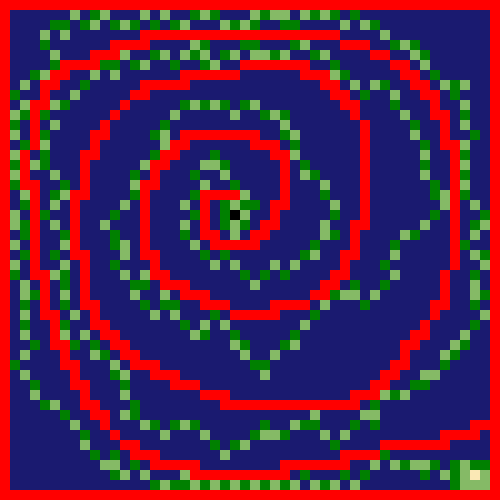
\includegraphics[width=0.5\textwidth]{./images/desarrollo/physarum/Circular1.png}}
        \caption{Physarum Polycephalum resolviendo un laberinto en espiral.} 
        \label{fig:physarumCircle1}    
    \end{figure}
    \begin{figure}[htbp]
        \centerline{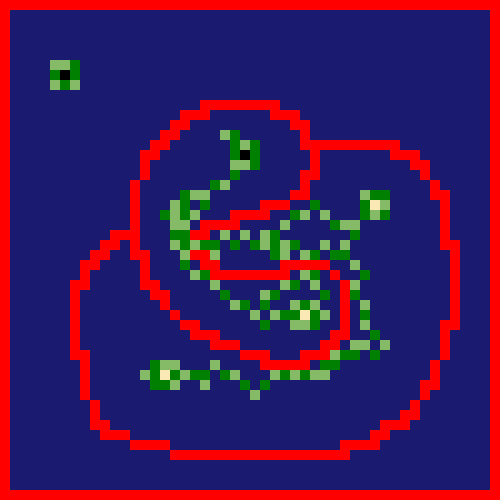
\includegraphics[width=0.5\textwidth]{./images/desarrollo/physarum/Random1.png}}
        \caption{Physarum Polycephalum resolviendo un laberinto de tipo circular.}
        \label{fig:physarumRandom1}    
    \end{figure}
    \begin{figure}[htbp]
        \centerline{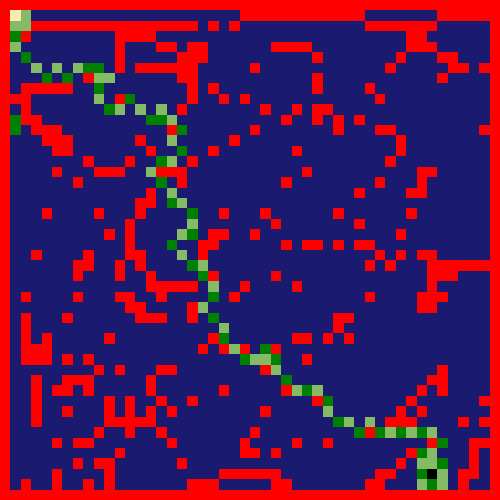
\includegraphics[width=0.5\textwidth]{./images/desarrollo/physarum/Obstaculos1.png}}
        \caption{Physarum Polycephalum resolviendo un laberinto con obst\'aculos.}
        \label{fig:physarumObstacles1}
    \end{figure}
    \vskip 0.5cm
    %P\'arrafo 3
    Gracias a la resoluci\'on de la fuga en las esquinas por nuestro algoritmo, es posible generar mapeos m\'as diversos 
        de cuevas y catacumbas. Este enfoque mejora significativamente nuestra comprensi\'on 
        de la topograf\'ia del \'area explorada. Adem\'as, la diversidad en el mapeo facilita la identificaci\'on 
        del n\'umero y variedad de caminos disponibles, lo que se ha implementado mediante un algoritmo de mapeo de im\'agenes que 
        ayuda en la representaci\'on gr\'afica de dicha topograf\'ia, como se muestra en la Figura \ref{fig:CaveSystemPhysarum}.
    \vskip 0.5cm
        \begin{figure}[htbp]
            \centerline{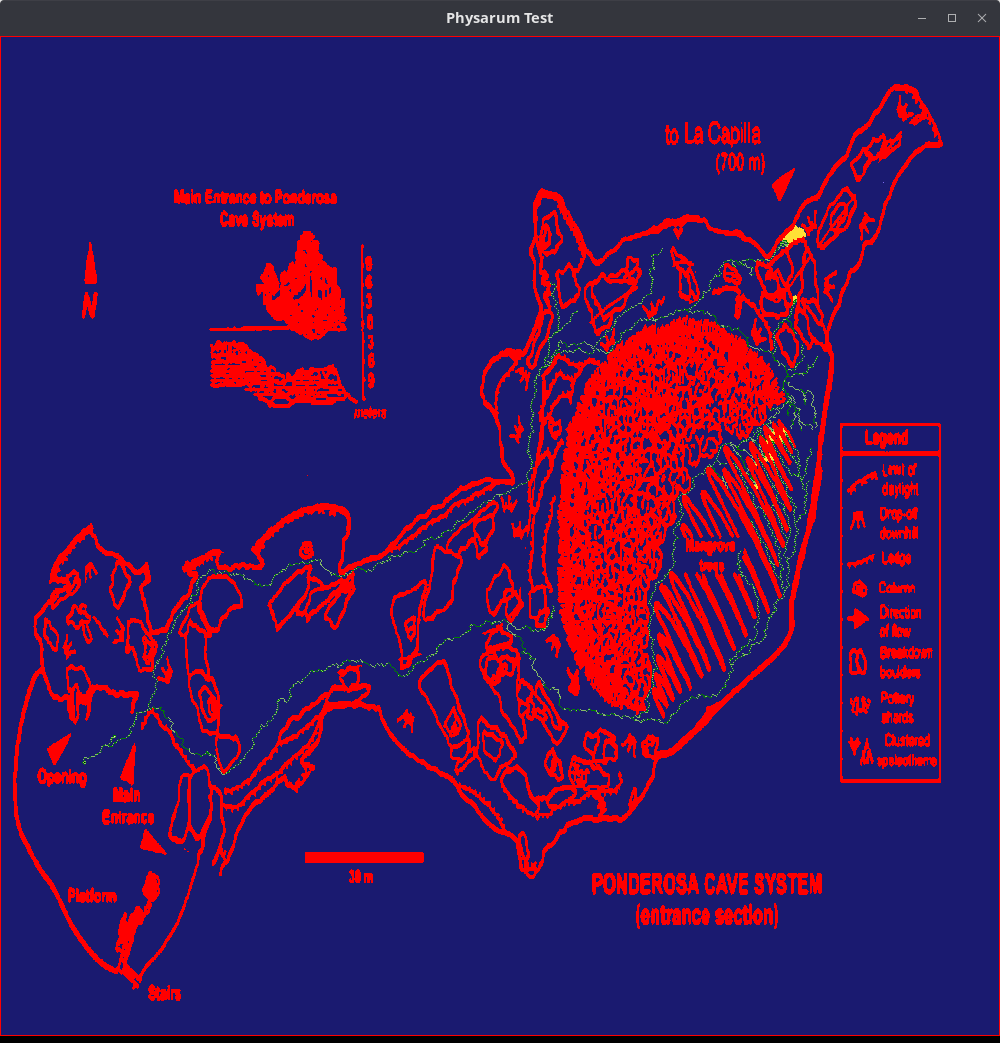
\includegraphics[width=0.40\textwidth]{./images/desarrollo/physarum/CaveSystemPhysarum.png}}
            \caption{Mapeo del sistema de cuevas usando Physarum Polycephalum.}
            \label{fig:CaveSystemPhysarum}
        \end{figure}
        \vskip 0.2cm
        Tambi\'en el algoritmo ha sido probado en un entorno real, donde ha sido capaz de generar 
            rutas \'optimas en la Catacumba de Par\'is, como se muestra en la Figura \ref{fig:Catacomb}. El espacio
            explorado por el algoritmo es de 1000 x 1000 c\'elulas.
        \vskip 0.2cm
        \begin{figure}[htbp]
            \centerline{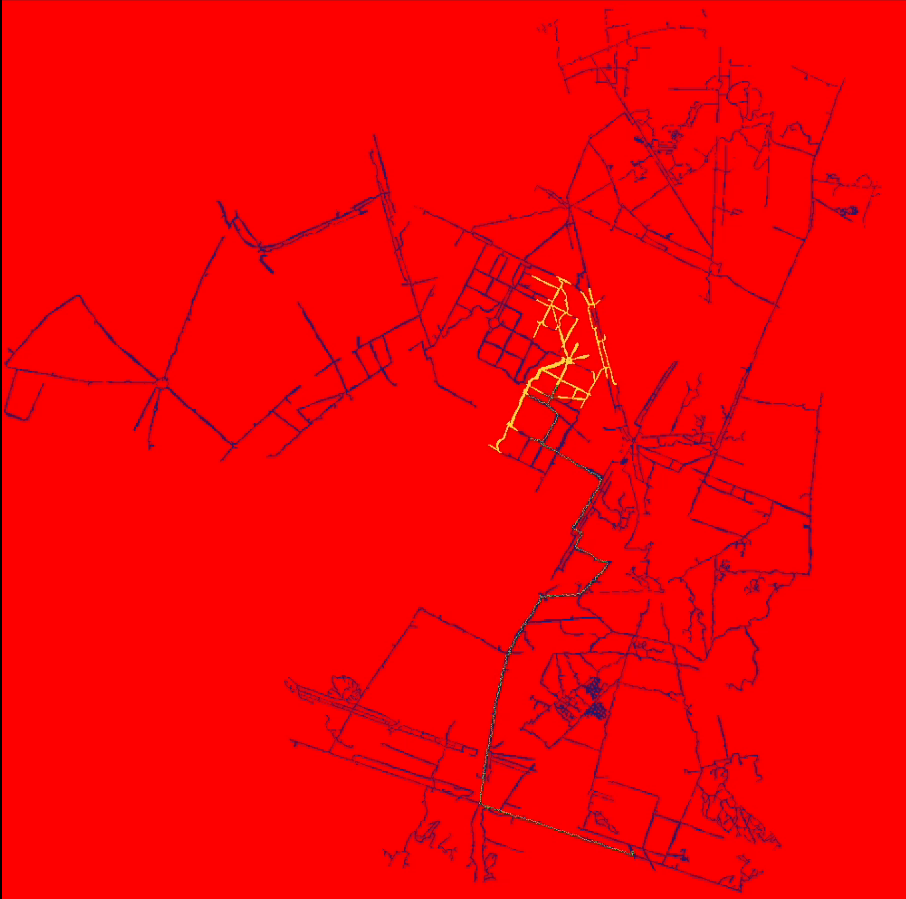
\includegraphics[width=0.75\textwidth]{./images/desarrollo/physarum/CatacoumbParis.png}}
            \caption{Mapeo de la catacumba usando Physarum Polycephalum, utiliza 5264 pasos para obtener la ruta.}
            \label{fig:Catacomb}
        \end{figure}
        %P\'arrafo 4
        \clearpage
        \vskip 0.5cm
        Como se puede observar en los Cuadros \ref{tab:estados02} y \ref{tab:estados03}, el algoritmo propuesto es capaz de resolver laberintos de manera eficiente, 
            generando rutas \'optimas en entornos complejos y desconocidos. Adem\'as, el algoritmo es capaz de adaptarse a diferentes topograf\'ias, 
            lo que lo convierte en una herramienta vers\'atil para la exploraci\'on de entornos desconocidos y nos es de ayuda en el monitoreo de poblaciones y sistemas relacionados.
        \vskip 0.5cm
        %P\'arrafo 5
        \begin{table}[h]
            \begin{center}
                \begin{tabular}{|c|c|c|}
                    \hline
                    \textbf{Color}&\textbf{State}&\textbf{Initial State Catacomb} \\
                    \hline
                    \cellcolor{blue} & 0 & 32,891  \\
                    \cellcolor{royalblue} & 1 & 1 \\
                    \cellcolor{red} & 2 & 967,105 \\
                    \cellcolor{black} & 3 & 2 \\
                    \cellcolor{yellow} & 4 & 0 \\
                    \cellcolor{darkgreen} & 5 & 0 \\
                    \cellcolor{lemon} & 6 & 0 \\
                    \cellcolor{darkgray} & 7 & 0 \\
                    \cellcolor{green} & 8 & 0 \\
                    \hline
                \end{tabular}
            \end{center}
            \caption{Estado inicial de la catacumba}
            \label{tab:estados02}
        \end{table}
        \begin{table}[h]
            \begin{center}
                \begin{tabular}{|c|c|c|}
                    \hline
                    \textbf{Color}&\textbf{State}&\textbf{Initial State Cave} \\
                    \hline
                    \cellcolor{blue} & 0 & 853,861  \\
                    \cellcolor{royalblue} & 1 & 3 \\
                    \cellcolor{red} & 2 & 146,135 \\
                    \cellcolor{black} & 3 & 1 \\
                    \cellcolor{yellow} & 4 & 0 \\
                    \cellcolor{darkgreen} & 5 & 0 \\
                    \cellcolor{lemon} & 6 & 0 \\
                    \cellcolor{darkgray} & 7 & 0 \\
                    \cellcolor{green} & 8 & 0 \\
                    \hline
                \end{tabular}
            \end{center}
            \caption{Estado inicial de la cueva}
            \label{tab:estados03}
        \end{table}
        Cabe se\~nalar que dado que el algoritmo est\'a bioinspirado, la funci\'on que simula el comportamiento del plasmodio 
            se asigna de manera pseudoaleatoria a un vecino adyacente, con una probabilidad de 1/8. Esta caracter\'istica permite 
            que la expansi\'on del algoritmo tome una forma circular en lugar de una expansi\'on cuadrada o lineal. Sin embargo, al 
            modificar la funci\'on de probabilidad, es posible lograr una expansi\'on m\'as irregular en lugar de simplemente circular.
        \clearpage
        En cuanto la implementaci\'on del algoritmo, se ha utilizado el lenguaje de programaci\'on C++ y la librer\'ia OpenCV para la 
            obtenci\'on de im\'agenes. La parte de las esquinas que mencionamos con anterioridad se implement\'o como se muestra en el Listing \ref{Script01}: 
        \begin{lstlisting}[language={C++}, caption={Implementaci\'on del problema de las esquinas}, label={Script01}]
            std::vector<int> Physarum::isOnCorner(std::vector<int> neighboursData) {
            std::vector<int> corners;
                if (neighboursData[0] == 2 && neighboursData[2] == 2) {
                    corners.push_back(1);
                }
                if (neighboursData[0] == 2 && neighboursData[6] == 2) {
                    corners.push_back(7);
                }
                if (neighboursData[6] == 2 && neighboursData[4] == 2) {
                    corners.push_back(5);
                }
                if (neighboursData[2] == 2 && neighboursData[4] == 2) {
                    corners.push_back(3);
                }
            return corners;
            }
        \end{lstlisting}
        %P\'arrafo 5
        En el Listing \ref{Script01}, se muestra la implementaci\'on de la funci\'on que detecta si el agente se encuentra en una esquina. 
            La funci\'on recibe un vector de enteros que representa los estados de los vecinos adyacentes. Si dos esquinas adyacentes 
            presentan repelentes, la funci\'on devuelve un vector con las esquinas en las que se encuentra el agente. 
            En caso contrario, la funci\'on devuelve un vector vac\'io.
        \vskip 0.5cm
        %P\'arrafo 6
        Por ello podemos decir que el algoritmo propuesto es capaz de resolver laberintos de manera eficiente, 
            generando rutas \'optimas en entornos complejos y desconocidos. Adem\'as, el algoritmo es capaz de 
            adaptarse a diferentes topograf\'ias, lo que lo convierte en una herramienta vers\'atil para la exploraci\'on 
            de entornos desconocidos y nos es de ayuda en el monitoreo de poblaciones y sistemas relacionados.
        \vskip 0.5cm
        %Generador de rutas de nuestro simulador
        \subsubsection{Generaci\'on de rutas de nuestro simulador} % (fold)
\label{ssub:subsubsection name}

    El robot de monitoreo deber\'a de seguir una ruta
        preestablecida, la cual es calculada por el algoritmo del
        Physarum Polycephalum en el simulador que ha sido
        desarrollado.
    \vskip 0.5cm
    Primeramente, se tiene un lienzo, el cual es representado por
        un arreglo de celdas de tama\~no n x n, donde n es el tama\~no
        deseado para la representaci\'on del espacio en el cual el
        Physarum calcular\'a la ruta una vez terminada la simulaci\'on
        de este.
    \vskip 0.5cm
    En el lienzo, se colocan los estados sobre el lienzo por medio
        del teclado y el mouse, donde en el teclado son presionadas
        las teclas de 1 al 9 para poder elegir cada uno de los estados
        que puede tomar la celda en la cual se haya presionado el
        bot\'on izquierdo del mouse. Los estados que tienen mayor
        relevancia y que son los que se deben de colocar para poder
        realizar la simulaci\'on correctamente son los 1 y 4, debido a
        que representan el nutriente como el punto inicial
        respectivamente. El punto inicial es de donde se empezar\'a
        con la expansi\'on del Physarum, mientras que el nutriente es
        el destino final, puesto que una vez encontrado, cambiara su
        estado al estado 6, el cual es correspondiente al estado de
        nutriente encontrado. Y una vez finalizada la simulaci\'on, el
        algoritmo se detendr\'a autom\'aticamente y quedar\'a plasmada
        la ruta por la cual el Physarum encontr\'o el o los nutrientes
        desde el punto inicial, la cual ser\'a enviada al robot para su
        posterior seguimiento para llegar a su destino en el mundo
        real.
    \vskip 0.5cm
    Al iniciar el programa, se despliega una pantalla la cual
        muestra el lienzo con el espacio que hemos predefinido
        anteriormente en el c\'odigo. En este espacio al inicio se
        pueden colocar los diferentes estados como se mencion\'o
        anteriormente, por lo que una vez se haya colocado la
        configuraci\'on deseada, para iniciar la simulaci\'on se presiona
        en el teclado la tecla ENTER. El algoritmo se empieza a
        expandir, siendo aplicadas cada una de las reglas en cada una
        de las celdas del arreglo. El algoritmo termina cuando la ruta
        es encontrada y el Physarum termina de contraerse, dicha
        ruta es la que es enviada al robot para su seguimiento.Primeramente, se iniciaron las simulaciones en espacios
        peque\~nos. La primera configuraci\'on creada fue la de un
        lienzo de tama\~no 10 x 10.
    \vskip 0.5cm
    %FIgura
    \begin{figure}[htbp]
        \centering
        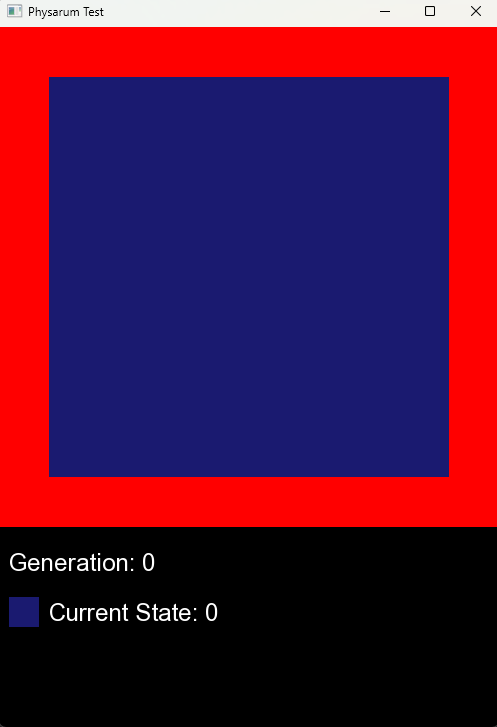
\includegraphics[width=0.5\textwidth]{./images/Pruebas/simulador/image001.png}
        \caption{Lienzo de 10 x 10}
        \label{fig:10x10}
    \end{figure}
    \vskip 0.5cm
    Posteriormente se colocaron los estados correspondientes a
    el estado inicial y al nutriente no encontrado.
    \vskip 0.5cm
    %FIgura
    \begin{figure}[htbp]
        \centering
        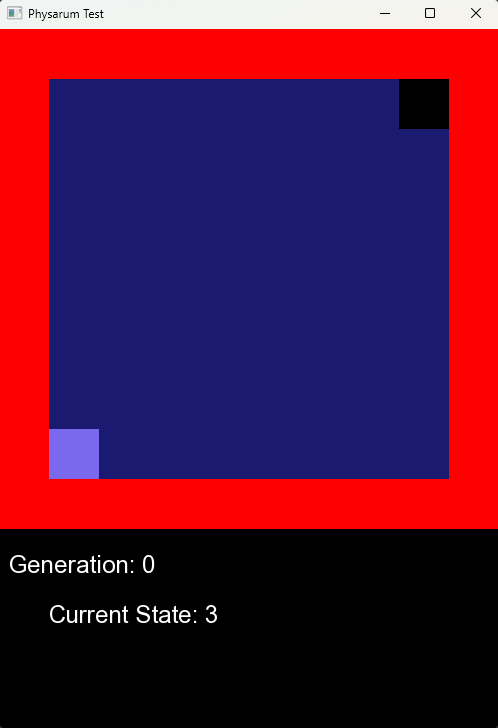
\includegraphics[width=0.5\textwidth]{./images/Pruebas/simulador/image002.png}
        \caption{Estados iniciales}
        \label{fig:Estados iniciales}
    \end{figure}
    \vskip 0.5cm
    Una vez colocada la configuraci\'on inicial, entonces se
        procede a iniciar la simulaci\'on, con la cual, al terminar las
        iteraciones se genera una ruta que va desde el estado inicial
        al nutriente no encontrado, el cual para este momento ha
        cambiado su estado a nutriente encontrado, cambiando a su
        vez el color correspondiente a este estado.
    \vskip 0.5cm
    %FIgura
    \begin{figure}[htbp]
        \centering
        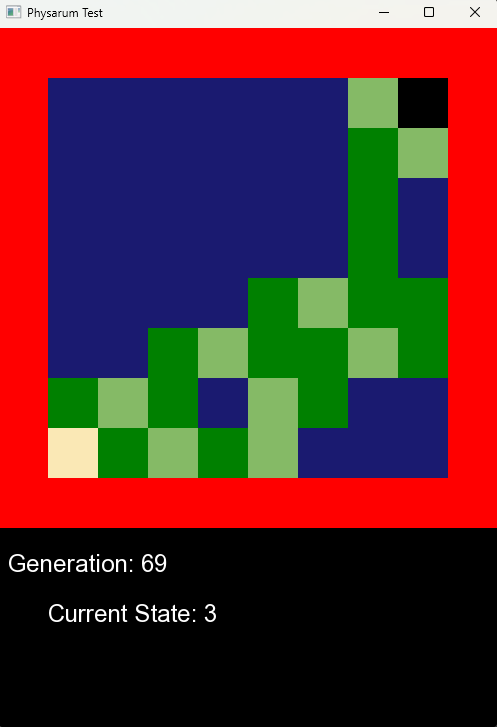
\includegraphics[width=0.5\textwidth]{./images/Pruebas/simulador/image003.png}
        \caption{Ruta encontrada}
        \label{fig:Ruta encontrada}
    \end{figure}
    \vskip 0.5cm
    En el programa es posible ver en qu\'e generaci\'on es en la que
        se encuentra el algoritmo, adem\'as del estado en el cual en ese
        momento se tiene elegido en el teclado, esto para ser
        colocado en el lienzo.
    \vskip 0.5cm
    Es posible colocar otra configuraci\'on una vez reiniciando el
        programa, donde se puede colocar los estados en distinta
        posici\'on, por lo que se muestran a continuaci\'on distintas
        configuraciones una vez finalizadas las simulaciones
        correspondientes a cada una de ellas.
    \vskip 0.5cm
    %FIgura
    \begin{figure}[htbp]
        \centering
        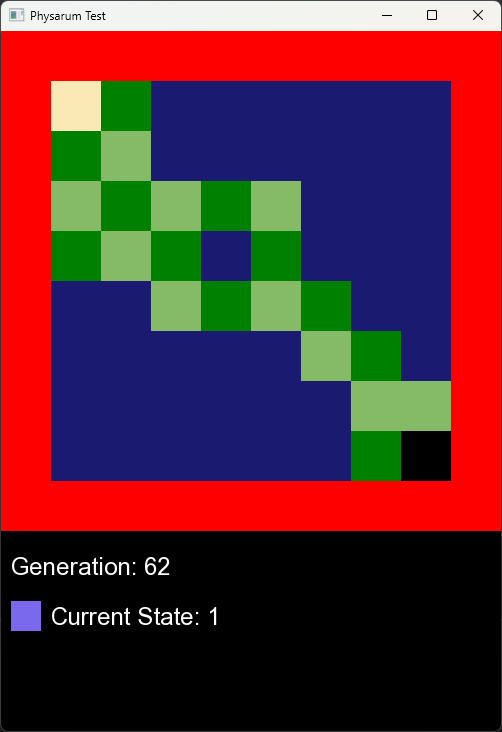
\includegraphics[width=0.5\textwidth]{./images/Pruebas/simulador/image004.png}
        \caption{Configuraci\'on 2}
        \label{fig:10x10}
    \end{figure}
    \vskip 0.5cm
    %FIgura
    \begin{figure}[htbp]
        \centering
        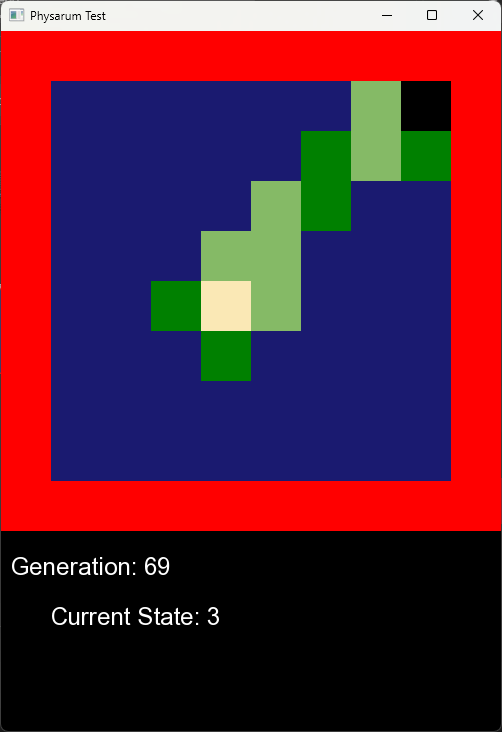
\includegraphics[width=0.5\textwidth]{./images/Pruebas/simulador/image005.png}
        \caption{Configuraci\'on 3}
        \label{fig:Estados iniciales}
    \end{figure}
    \vskip 0.5cm
    %FIgura
    \begin{figure}[htbp]
        \centering
        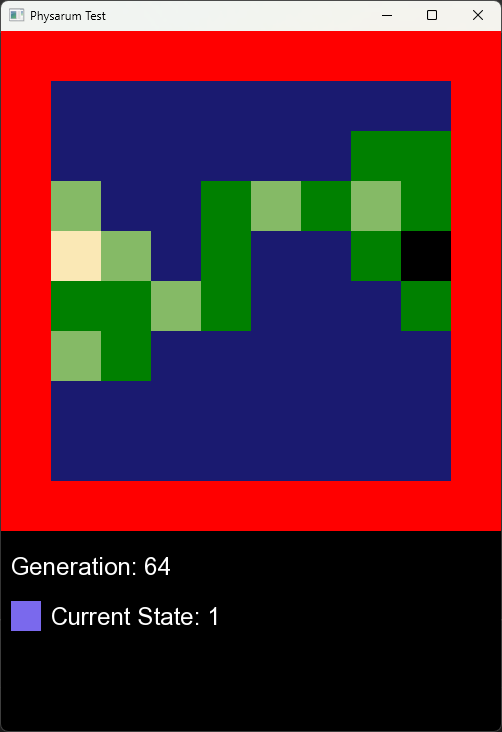
\includegraphics[width=0.5\textwidth]{./images/Pruebas/simulador/image006.png}
        \caption{Configuraci\'on 4}
        \label{fig:Ruta encontrada}
    \end{figure}
    \vskip 0.5cm
    Las simulaciones realizadas nos han devuelto resultados
        satisfactorios, debido a que las rutas son correctamente
        generadas de acuerdo a las reglas plasmadas en el algoritmo,
        yendo del punto inicial al final, y finalizando una vez que el
        Physarum ya no tiene la necesidad de expandirse, debido a
        que ha encontrado el nutriente que estaba buscando.
    \clearpage
% subsubsection subsubsection name (end)
        \subsubsection{Codificaci\'on e implementaci\'on de algoritmo en el robot en la primera iteraci\'on 1} % (fold)
\label{ssub:Codi}
    Con las rutas que han sido generadas de acuerdo a cada una
        de las simulaciones que fueron ejecutadas en el programa,
        como ya se ha mencionado, se genera la informaci\'on con la
        cual el robot realizar\'a el seguimiento de esta ruta para llegar
        de un punto inicial al final. Esta informaci\'on corresponde a
        la ruta que genera el Physarum cuando termina la simulaci\'on
        de llegar desde su punto inicial de expansi\'on a un nutriente
        con el cual se alimenta.
    \vskip 0.5cm
    Para poder hacer una correcta manipulaci\'on de la
        informaci\'on, la cual pueda ser enviada al robot que este
        pueda interpretarla y avanzar de acuerdo la ruta generada, es
        necesario crear un espacio el cual represente la posici\'on del
        robot en un determinado lugar, junto con el destino al cual se
        quiere llegar, a partir de ah\'i pasar esta configuraci\'on al
        modelo del Physarum, ejecutar la simulaci\'on y obtener la
        ruta, finalizando con la recopilaci\'on de la informaci\'on
        relacionada con la ruta y su almacenamiento, lo cual es
        representado en el Listing \ref{Script02}.
    \vskip 0.5cm
    
    \begin{lstlisting}[language={PseudoCode}, caption={Pseudo C\'odigo de las rutas}, label={Script02}]
    Iniciar programa
    Colocar la configuraci\'on inicial
    Coloca punto inicial
    Coloca punto final
    Ejecutar Simulador_Physarum
    Si Simulador_Physarum obtuvo ruta, entonces:
        Guardar las coordenadas del punto inicial
        Guardar las coordenadas del punto final
        Guardar las coordenadas de las c\'elulas por orden de aparici\'on
        Desplegar todas las coordenadas en un archivo
    Si no
        Finaliza programa
    Fin Si
    \end{lstlisting}
    \vskip 0.5cm
    A partir de lo anterior, se comprende que al robot se le ser\'a
        enviado las coordenadas correspondientes a la ruta obtenida
        por el simulador del Physarum, con un punto inicial, el cual
        marcar\'a su posici\'on actual, su punto final, representando el
        destino al cual llegar\'a el robot y las c\'elulas del Physarum
        ordenadas por orden de aparici\'on, las cuales son las
        coordenadas por las cuales el robot tendr\'a que pasar para
        llegar desde el punto inicial al final.
    \vskip 0.5cm
    Con lo anterior, es posible la creaci\'on de informaci\'on la cual
        el robot sea capaz de leer y a partir de sus propias funciones,
        llegar de un punto inicial al final. Esta informaci\'on es
        almacenada en un archivo, el cual contiene cada una de las
        coordenadas ordenadas, siendo la primera el punto inicial,
        posteriormente cada una de las dem\'as coordenadas que
        representan a cada una de las c\'elulas del Physarum,
        ordenadas por orden de aparici\'on para que el robot tenga un
        orden el cual seguir para poder llegar a su destino.
    \vskip 0.5cm
    Finalmente, la \'ultima coordenada corresponde a la
        coordenada del punto final, el cual es el destino al cual el
        robot deber\'a de llegar, finalizando as\'i su recorrido.
        
% subsubsection Codi (end)
        \subsubsection{Codificaci\'on e implementaci\'on de algoritmo en el robot en la primera iteraci\'on 2}
    La implementaci\'on en el robot no cambia respecto a c\'omo se
        estuvo planeando desde el inicio, debido a que las rutas son
        obtenidas de acuerdo con la simulaci\'on del Physarum, que,
        una vez finalizada esta, a partir de una serie de condiciones y
        convirtiendo el camino en coordenadas las cuales el robot
        pueda interpretar para realizar su recorrido de la mejor forma
        posible, se pueda llegar de un punto inicial a un punto final
        de forma correcta.
        \vskip 0.5cm
    Como se plante\'o desde el inicio, el algoritmo debe generar
        su ruta con ayuda del Physarum, y a partir de esta, generar
        una serie de coordenadas las cuales el robot pueda seguir
        para moverse de un punto al otro. En la implementaci\'on, el
        archivo generado a partir de la ruta que se obtuvo con el
        Physarum, se puede ver en la Figura \ref{fig:Archivoderutas01}.
    \vskip 0.5cm
    %imagen
    \begin{figure}[htbp]
        \centering
        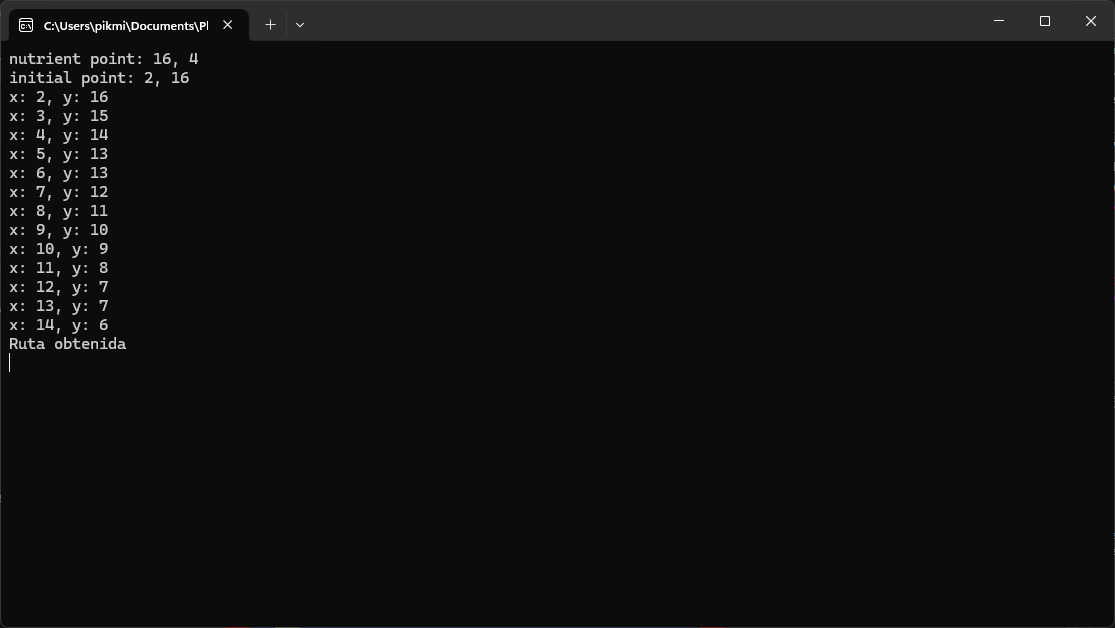
\includegraphics[width=0.5\textwidth]{./images/Pruebas/simulador/image043.png}
        \caption{Archivo de rutas}
        \label{fig:Archivoderutas01}
    \end{figure}
    \vskip 0.5cm
    Las coordenadas est\'an dadas de acuerdo con el punto de
        partida, que est\'a representado a partir del punto inicial en el
        simulador, hasta el destino, el cual es uno de los nutrientes
        en el simulador del Physarum y son de vital importancia para
        poder generar la ruta, ya que, con la ausencia de estos, no se
        puede generar una ruta. Las coordenadas est\'an ordenadas deforma de aparici\'on, lo que hace que haya una forma de
        seguirla correctamente y no se deba de perder, o seguir la
        ruta de manera err\'onea.
        \subsubsection{Ajustes del algoritmo basados en pruebas unitarias 1}
    Recopilando los datos obtenidos en algunas de las pruebas
        unitarias realizadas hasta el momento de realizaci\'on de estas
        mismas, se aplicaron algunos cambios al programa,
        principalmente enfocados a mejorar cada una de sus
        funciones y que sea mucho m\'as f\'acil en cuanto a la calidad
        del algoritmo.
        \vskip 0.5cm
    Los cambios que han sido aplicados hasta el momento
        corresponden a los siguientes elementos que conforman el
        programa:
        \vskip 0.5cm
    %figura
    \begin{figure}[htbp]
        \centering
        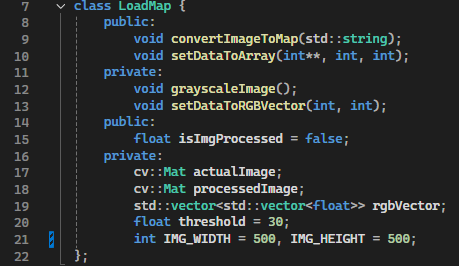
\includegraphics[width=0.5\textwidth]{./images/Pruebas/simulador/image045.png}
        \caption{Implementaci\'on del LoadMap}
        \label{fig:Pruebaunitaria2}
    \end{figure}
    Implementaci\'on de la clase LoadMap: A pesar de que se
        pueda configurar un espacio en el lienzo por medio del
        dibujo, muchas veces al querer colocar un croquis o un mapa
        de determinado espacio, dibujar a mano con el rat\'on resulta
        poco conveniente, por lo que se implement\'o la clase
        LoadMap, la cual hace uso de la librer\'ia OpenCV,
        transformando una imagen en un dibujo en el lienzo del
        programa al inicializarse este \'ultimo. Esto se puede ver en
        la Figura \ref{fig:Pruebaunitaria2}.
        \vskip 0.5cm
    %figura
    \begin{figure}[htbp]
        \centering
        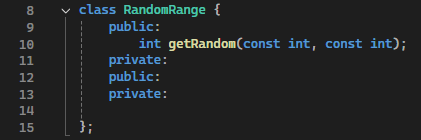
\includegraphics[width=0.5\textwidth]{./images/Pruebas/simulador/image046.png}
        \caption{Clase RandomRange}
        \label{fig:Pruebaunitaria3}
    \end{figure}
    Clase RandomRange: Al realizarse las primeras pruebas
        unitarias en el software, fue obtenido como resultado que es
        poco conveniente usar la funci\'on rand() debido a que tiende
        a ser mucho m\'as lenta que otras implementaciones, adem\'as
        de que su aleatoriedad no es la mejor y adem\'as, no es
        multihilo, lo que impide que si en el futuro el algoritmo se
        quiere paralelizar, esto dificulte la implementaci\'on de n\'umero randoms que sean thread safe. Esto se puede ver en
        la Figura \ref{fig:Pruebaunitaria3}.
        \vskip 0.5cm

        \subsubsection{Ajustes del algoritmo basados en pruebas unitarias 2}
%Parrafo 1
    En esta ocasi\'on, no se realizaron cambios en el algoritmo,
        debido a que se pudo comprobar el correcto funcionamiento
        de este mismo y la cuesti\'on real de funcionamiento o
        pruebas es el cambio de configuraciones en el estado inicial
        para la obtenci\'on de rutas, siendo evaluados distintos casos y
        configuraciones del estado inicial.
    \vskip 0.5cm
    Debido a que hasta el momento el algoritmo cumple su
        funci\'on y las pruebas unitarias no revelaron alg\'un resultado
        en el cual haya alg\'un error o falla con alguna parte del
        algoritmo, en esta ocasi\'on los ajustes al algoritmo no fueron
        realizados.
    \vskip 0.5cm
    Es importante recalcar que el funcionamiento base del
        algoritmo es importante para la funcionalidad de la
        simulaci\'on en general, esto debido a que un peque\~no cambio
        a alguna de sus partes puede alterar el resultado general y
        formar comportamientos o generar resultados no deseados y
        que no logran cumplir el objetivo general del software el
        cual es la generaci\'on de rutas a partir del organismo
        Physarum.
        \subsubsection{Dise\~no inicial de interfaz para control y monitorear}
    Para el dise\~no de la interfaz en la cual se puede controlar y a
        su vez, hacer uso del sistema de monitoreo del robot, es
        necesario conocer cada uno de los componentes que son
        necesarios mostrar y los que ser\'an necesarios para realizar la
        funcionalidad correspondiente, los cuales corresponden a los
        siguientes:
    \vskip 0.5cm
    Sistema de monitoreo: La interfaz debe mostrar la visi\'on de
        la c\'amara que esta incorporada al robot, por lo que debe de
        haber un espacio dedicado a mostrar a esta misma.
        \vskip 0.5cm
    Sistema LiDAR: En la interfaz tambi\'en se debe mostrar cada
        uno de los puntos que son obtenidos a trav\'es de este sistema,
        los cuales representan los obst\'aculos que est\'an siendo
        detectados por el robot, as\'i como una representaci\'on de lo
        que se encuentra alrededor de \'este.
        \vskip 0.5cm
    M\'odulo de navegaci\'on: Debido a que el robot puede ser
        controlado a distancia, se necesita de la colocaci\'on de una
        serie de botones con los cuales el robot pueda realizar lanavegaci\'on b\'asica
        Con los componentes mencionados anteriormente, se realiza
        el dise\~no de la interfaz inicial con la cual cada uno de estos
        es colocado de tal forma que se tenga acceso a \'el y se
        puedan realizar cada una de las tareas que fueron explicadas
        anteriormente.
    \vskip 0.5cm
    %imagen
    \begin{figure}[htbp]
        \centering
        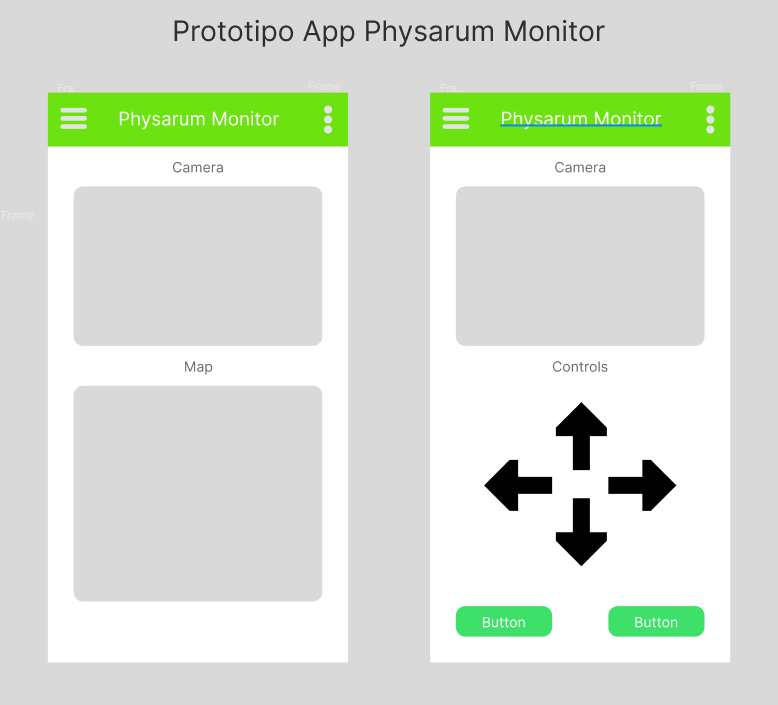
\includegraphics[width=0.5\textwidth]{./images/Pruebas/simulador/image077.png}
        \caption{Prototipo App Physarum Monitor}
        \label{fig:77}
    \end{figure}
    \vskip 0.5cm
    Con la disposici\'on mostrada, podemos ver que se colocan
        los elementos que son necesarios para poder cumplir con
        cada una de las funciones que son necesarias para el control
        y monitoreo del robot. Se muestran dos configuraciones, una
        de las cuales contiene tanto la vista de la c\'amara, as\'i como
        de la vista de la informaci\'on que se nos es enviada por parte
        del robot, la cual es obtenida con el sensor LiDAR. La
        siguiente configuraci\'on contiene tanto la vista de la c\'amara
        del robot, como una serie de botones los cuales representan
        cada uno de los movimientos con los cuales es posible
        controlar al robot. Esta configuraci\'on en particular est\'a
        dise\~nada para poder observar por medio de la c\'amara los
        movimientos que se est\'an realizando a trav\'es de los botones
        y as\'i, tener una mejor noci\'on de lo que se est\'a haciendo con
        el robot, as\'i como para poder orientarse y poder tener un
        mejor control de este robot.
        \subsubsection{Ajustes de rutas basado en resultado de pruebas de aceptaci\'on 1}
    Con los resultados que fueron obtenidos a partir de la
        ejecuci\'on de las pruebas de aceptaci\'on, se toma en cuenta
        que hay algunas configuraciones o ajustes que se deben de
        hacer al algoritmo. Una de las primeras es generar una ruta
        'mas limpia', es decir, una ruta en la cual existan mucho
        menos celdas las cuales impidan o dificulten generar una
        ruta un poco m\'as optima o que causan algunos
        impedimentos a la hora de generar el ordenamiento de
        coordenadas para ser enviadas al robot para la realizaci\'on de
        su funcionalidad de llegar a su destino.    
    \vskip 0.5cm
    Una de las soluciones que se considera para poder obtener
        las rutas un poco m\'as limpias y ajustarlas es limpiar un poco
        el camino o ruta generada por el Physarum una vez esta
        \'ultima siendo obtenida es eliminar las c\'elulas que conforman
        al estado 8 y 5 respectivamente, las cuales no sean
        necesarias para el c\'alculo de la ruta o que no formen parte
        importante de la ruta que fue obtenida. Para esto se
        consideran dos casos importantes
    \vskip 0.5cm
    \begin{enumerate}
        \item Las c\'elulas alrededor de el punto inicial y el punto
            final.
        \item Las c\'elulas que no conectan una c\'elula con otra.
    \end{enumerate}
    \vskip 0.5cm
    Una de las ideas para poder eliminar estas c\'elulas las cuales
        dificultan la obtenci\'on correcta de las rutas es eliminar las
        c\'elulas que est\'an alrededor del estado inicial y el estado
        final, dejando \'unicamente las que tienen conexi\'on con otras
        c\'elulas las cuales pertenecen a la ruta general.
    \vskip 0.5cm
    Esto se realiz\'o de la siguiente forma creando un nuevo
        aut\'omata con las siguientes reglas:
    \vskip 0.5cm
    \begin{itemize}
        \item Si el estado es 1 y alrededor no hay ning\'un estado 1, entonces es estado 0, sino, es estado 1.
        \item Si el estado es 2 y alrededor no hay ning\'un estado 1, entonces es estado 0, sino, es estado 2.
        \item Si el estado es 3, entonces es estado 7.
        \item Si el estado es 4 y alrededor no hay ning\'un estado 1, entonces es estado 0, sino, es estado 4.
        \item Si el estado es 5 y alrededor hay un punto inicial, entonces es estado 2, sino, si alrededor hay un nutriente, entonces es estado 4, sino es estado 1.
        \item Si es estado 6, entonces es estado 9.
        \item Si es estado 7, se queda en estado 7.
        \item Si el estado es 8 y alrededor hay un punto inicial, entonces es estado 2, sino, si alrededor hay un nutriente, entonces es estado 4, sino es estado 1.
        \item Si es estado 9, entonces se queda en estado 9.
    \end{itemize}
    \vskip 0.5cm    
    Y queda plasmado con el siguiente c\'odigo:
    \vskip 0.5cm
    \begin{lstlisting}[language={C++}, caption={Ruta Ajuste 1}, label={Script}]
        switch (tab[i][j]) {
            case 1:
                if (!aroundState1)
                    cellsAux[i][j] = 0;
                else
                    cellsAux[i][j] = 1;
            break;
            case 2:
                if (!aroundState1)
                    cellsAux[i][j] = 0;
                else
                    cellsAux[i][j] = 2;
            break;
            case 3:
                cellsAux[i][j] = 7;
            break;
            case 4:
                if (!aroundState1)
                    cellsAux[i][j] = 0;
                else
                    cellsAux[i][j] = 4;
            break;
            case 5:
                cellsCounter++;
                if (isInitialPointAround)
                    cellsAux[i][j] = 2;
                else if (isNutrientAround)
                    cellsAux[i][j] = 4;
                else
                    cellsAux[i][j] = 1;
            break;
            case 6:
                cellsAux[i][j] = 9;
            break;
            case 7:
                cellsAux[i][j] = 7;
            break;
            case 8:
                cellsCounter++;
                if (isInitialPointAround)
                    cellsAux[i][j] = 2;
                else if(isNutrientAround)
                    cellsAux[i][j] = 4;
                else
                    cellsAux[i][j] = 1;
            break;
            case 9:
                cellsAux[i][j] = 9;
            break;
        }
    \end{lstlisting}
    % section Resultados de las pruebas (end)
\vskip 0.5cm
    Lo anterior se hace para poder obtener una ruta con una
        mejor claridad y que dificulte menos el ordenamiento y la
        manera en la cual se obtienen las coordenadas con las cuales
        se realiza el recorrido.
% subsection subsection name (end)